\documentclass[xcolor=x11names, svgnames, rgb]{beamer}

\setbeamertemplate{navigation symbols}{}
\setbeamercolor{block title}{bg=blue!40}
\setbeamercolor{block body}{bg=blue!20}

%% Beamer Layout %%%%%%%%%%%%%%%%%%%%%%%%%%%%%%%%%%
\useoutertheme[subsection=false,shadow]{miniframes}
\useinnertheme{default}
\usefonttheme{serif}
\usepackage{palatino}
\setbeamerfont{title like}{shape=\scshape}
\setbeamerfont{frametitle}{shape=\scshape}
\setbeamercolor*{lower separation line head}{bg=DeepSkyBlue4}
\setbeamercolor*{normal text}{fg=black,bg=white}
\setbeamercolor*{alerted text}{fg=red}
\setbeamercolor*{example text}{fg=black}
\setbeamercolor*{structure}{fg=black}
\setbeamercolor*{palette tertiary}{fg=black,bg=black!10}
\setbeamercolor*{palette quaternary}{fg=black,bg=black!10}
%% END Beamer Layout %%%%%%%%%%%%%%%%%%%%%%%%%%%%%%%%%%%%%%%%%%%%
\usepackage{graphicx}
\usepackage{algpseudocode}
\usepackage{soul}

\usepackage{mathtools}
\newcommand{\defeq}{\vcentcolon=}
\DeclarePairedDelimiter{\paren}{(}{)}

\newcommand{\dec}{\operatorname{dec}}
\newcommand{\poly}{\operatorname{poly}}
\newcommand{\polylog}{\operatorname{polylog}}
\newcommand{\github}{\url{github.com/awestover/Parallel-Partition}}
\newcommand{\defn}[1]       {{\textit{\textbf{\boldmath #1}}}}
\newcommand{\paragraph}[1]{\vspace{0.09in}\noindent{\bf \boldmath #1.}} 
\usepackage{amsmath}
\def\E{\operatorname{\mathbb{E}}}
\usepackage{amssymb}
\usepackage{amsthm}

\newtheorem{proposition}{Proposition}
\newtheorem{defin}{Definition}
\newtheorem{conj}{Conjecture}

\usepackage{hyperref}

\usepackage{tikz,pgfplots}
\usepackage{etoolbox}
%% This makes the colors annoyingly bright, but at least they're easy to distinguish.
\pgfplotsset{
  every  tick/.style={red,}, minor x tick num=1,
  cycle list={teal,every mark/.append style={fill=teal!80!black},mark=*\\%
orange,every mark/.append style={fill=orange!80!black},mark=square*\\%
cyan!60!black,every mark/.append style={fill=cyan!80!black},mark=otimes*\\%
red!70!white,mark=star\\%
lime!80!black,every mark/.append style={fill=lime},mark=diamond*\\%
red,densely dashed,every mark/.append style={solid,fill=red!80!black},mark=*\\%
yellow!60!black,densely dashed,
every mark/.append style={solid,fill=yellow!80!black},mark=square*\\%
black,every mark/.append style={solid,fill=gray},mark=otimes*\\%
blue,densely dashed,mark=star,every mark/.append style=solid\\%
red,densely dashed,every mark/.append style={solid,fill=red!80!black},mark=diamond*\\%
}
}
\pgfplotsset{compat=1.6}


\usepackage{xcolor}
\newcommand{\citefont}[1]{{\tiny \textcolor{Gray}{#1}}}


\title{The Variable Processor Cup Game}
\author{Alek Westover}
\institute{Belmont High School}
\date{June 7, 2020}

\begin{document}
 
\frame{\titlepage}

\begin{frame}[t]{What is the Cup Game?}
  \begin{definition}
  \defn{$p$-processor cup-game} on $n$ cups: \\
  multi-round game \\
  on each round:
  \begin{itemize}
    \item The \defn{filler} distributes $p$ units of water among the cups \\(with at most $1$ unit to any particular cup)
    \item Then the \defn{emptier} chooses $p$ cups to remove (at most) one unit of water from
  \end{itemize}
  \end{definition}

  \vspace{0.4cm}
  Note: \\
  Emptier must allocate resources discretely\\
  Filler can allocate resources continuously
\end{frame}

\begin{frame}[t]{What is the Cup Game?}
  \begin{definition}
    \defn{Backlog}:\\
  Amount of water in the fullest cup
  \end{definition}
  \vspace{0.4cm}

  Emptier tries to \emph{minimize} backlog\\
  Filler tries to \emph{maximize} backlog
\end{frame}

\begin{frame}[t]{Why is the Cup Game Important?}
  Models \defn{work scheduling}:
  \begin{itemize}
    \item Cups represent tasks
    \item At each time step:
      \begin{itemize}
        \item new work comes in, distributed arbitrarily among the tasks
        \item $p$ processors are allocated to work on a subset of the tasks
      \end{itemize}
\end{itemize}

  \vspace{0.5cm}
  Also an interesting mathematical object
\end{frame}

\begin{frame}[t]{Analysis of the cup game}
  Prove \defn{upper bounds} and \defn{lower bounds} on backlog.

\end{frame}

\begin{frame}[t]{Single-Processor Lower Bound}
  \textbf{Filling strategy}: \\Distribute water equally amongst cups not yet emptied from.
  \vspace{0.3cm}

  \begin{overprint}
    \onslide<1>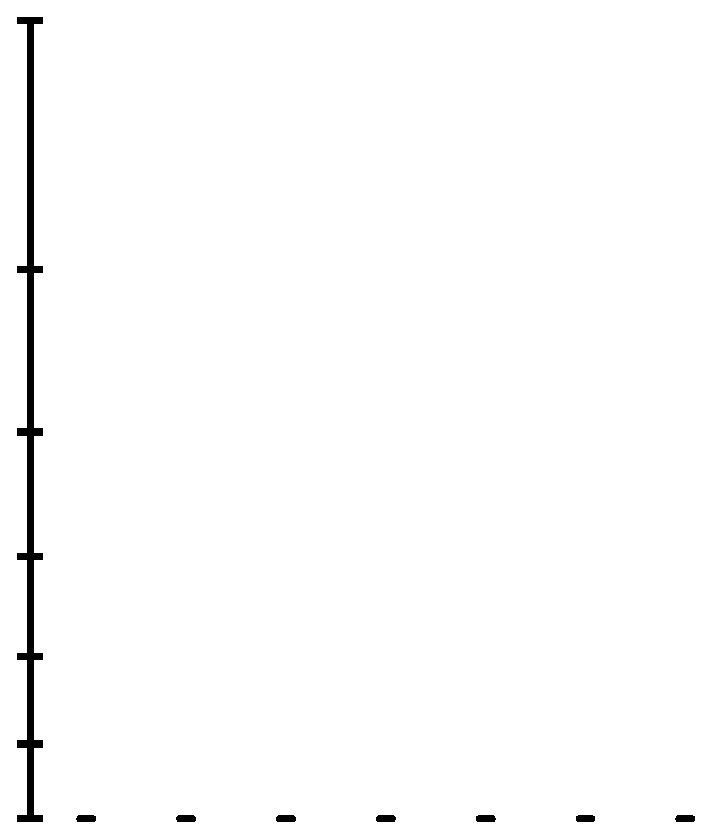
\includegraphics[width=0.5\linewidth]{singleProcessorLowerBound/round_0_1.eps}
    \onslide<2>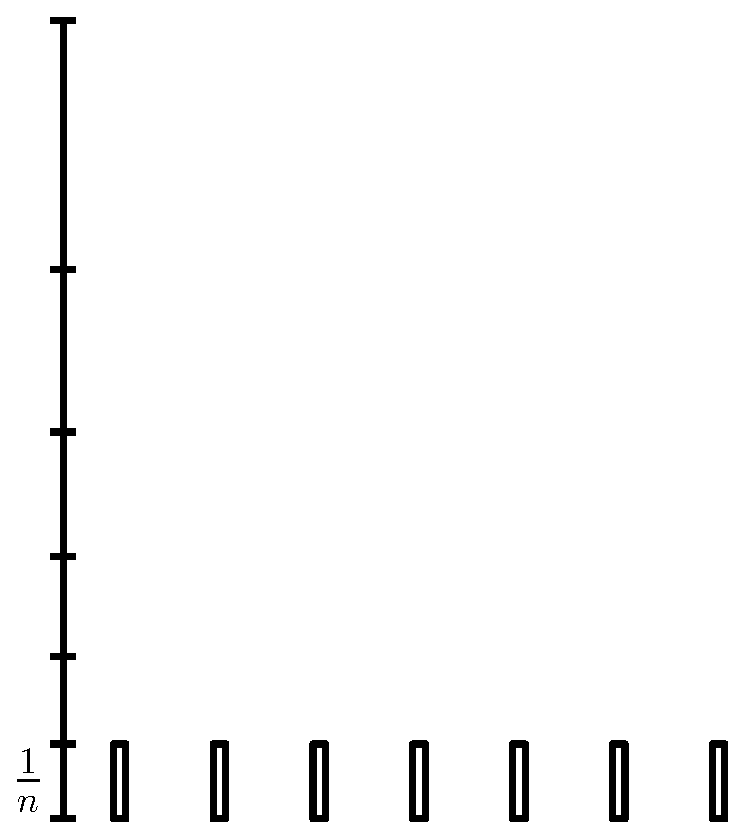
\includegraphics[width=0.5\linewidth]{singleProcessorLowerBound/round_1_0.eps}
    \onslide<3>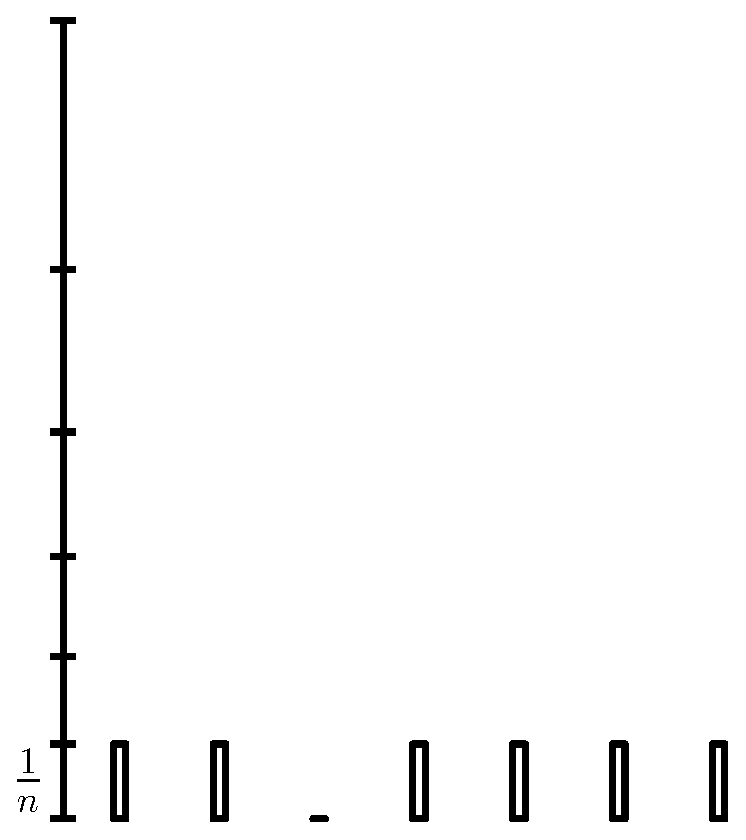
\includegraphics[width=0.5\linewidth]{singleProcessorLowerBound/round_1_1.eps}
    \onslide<4>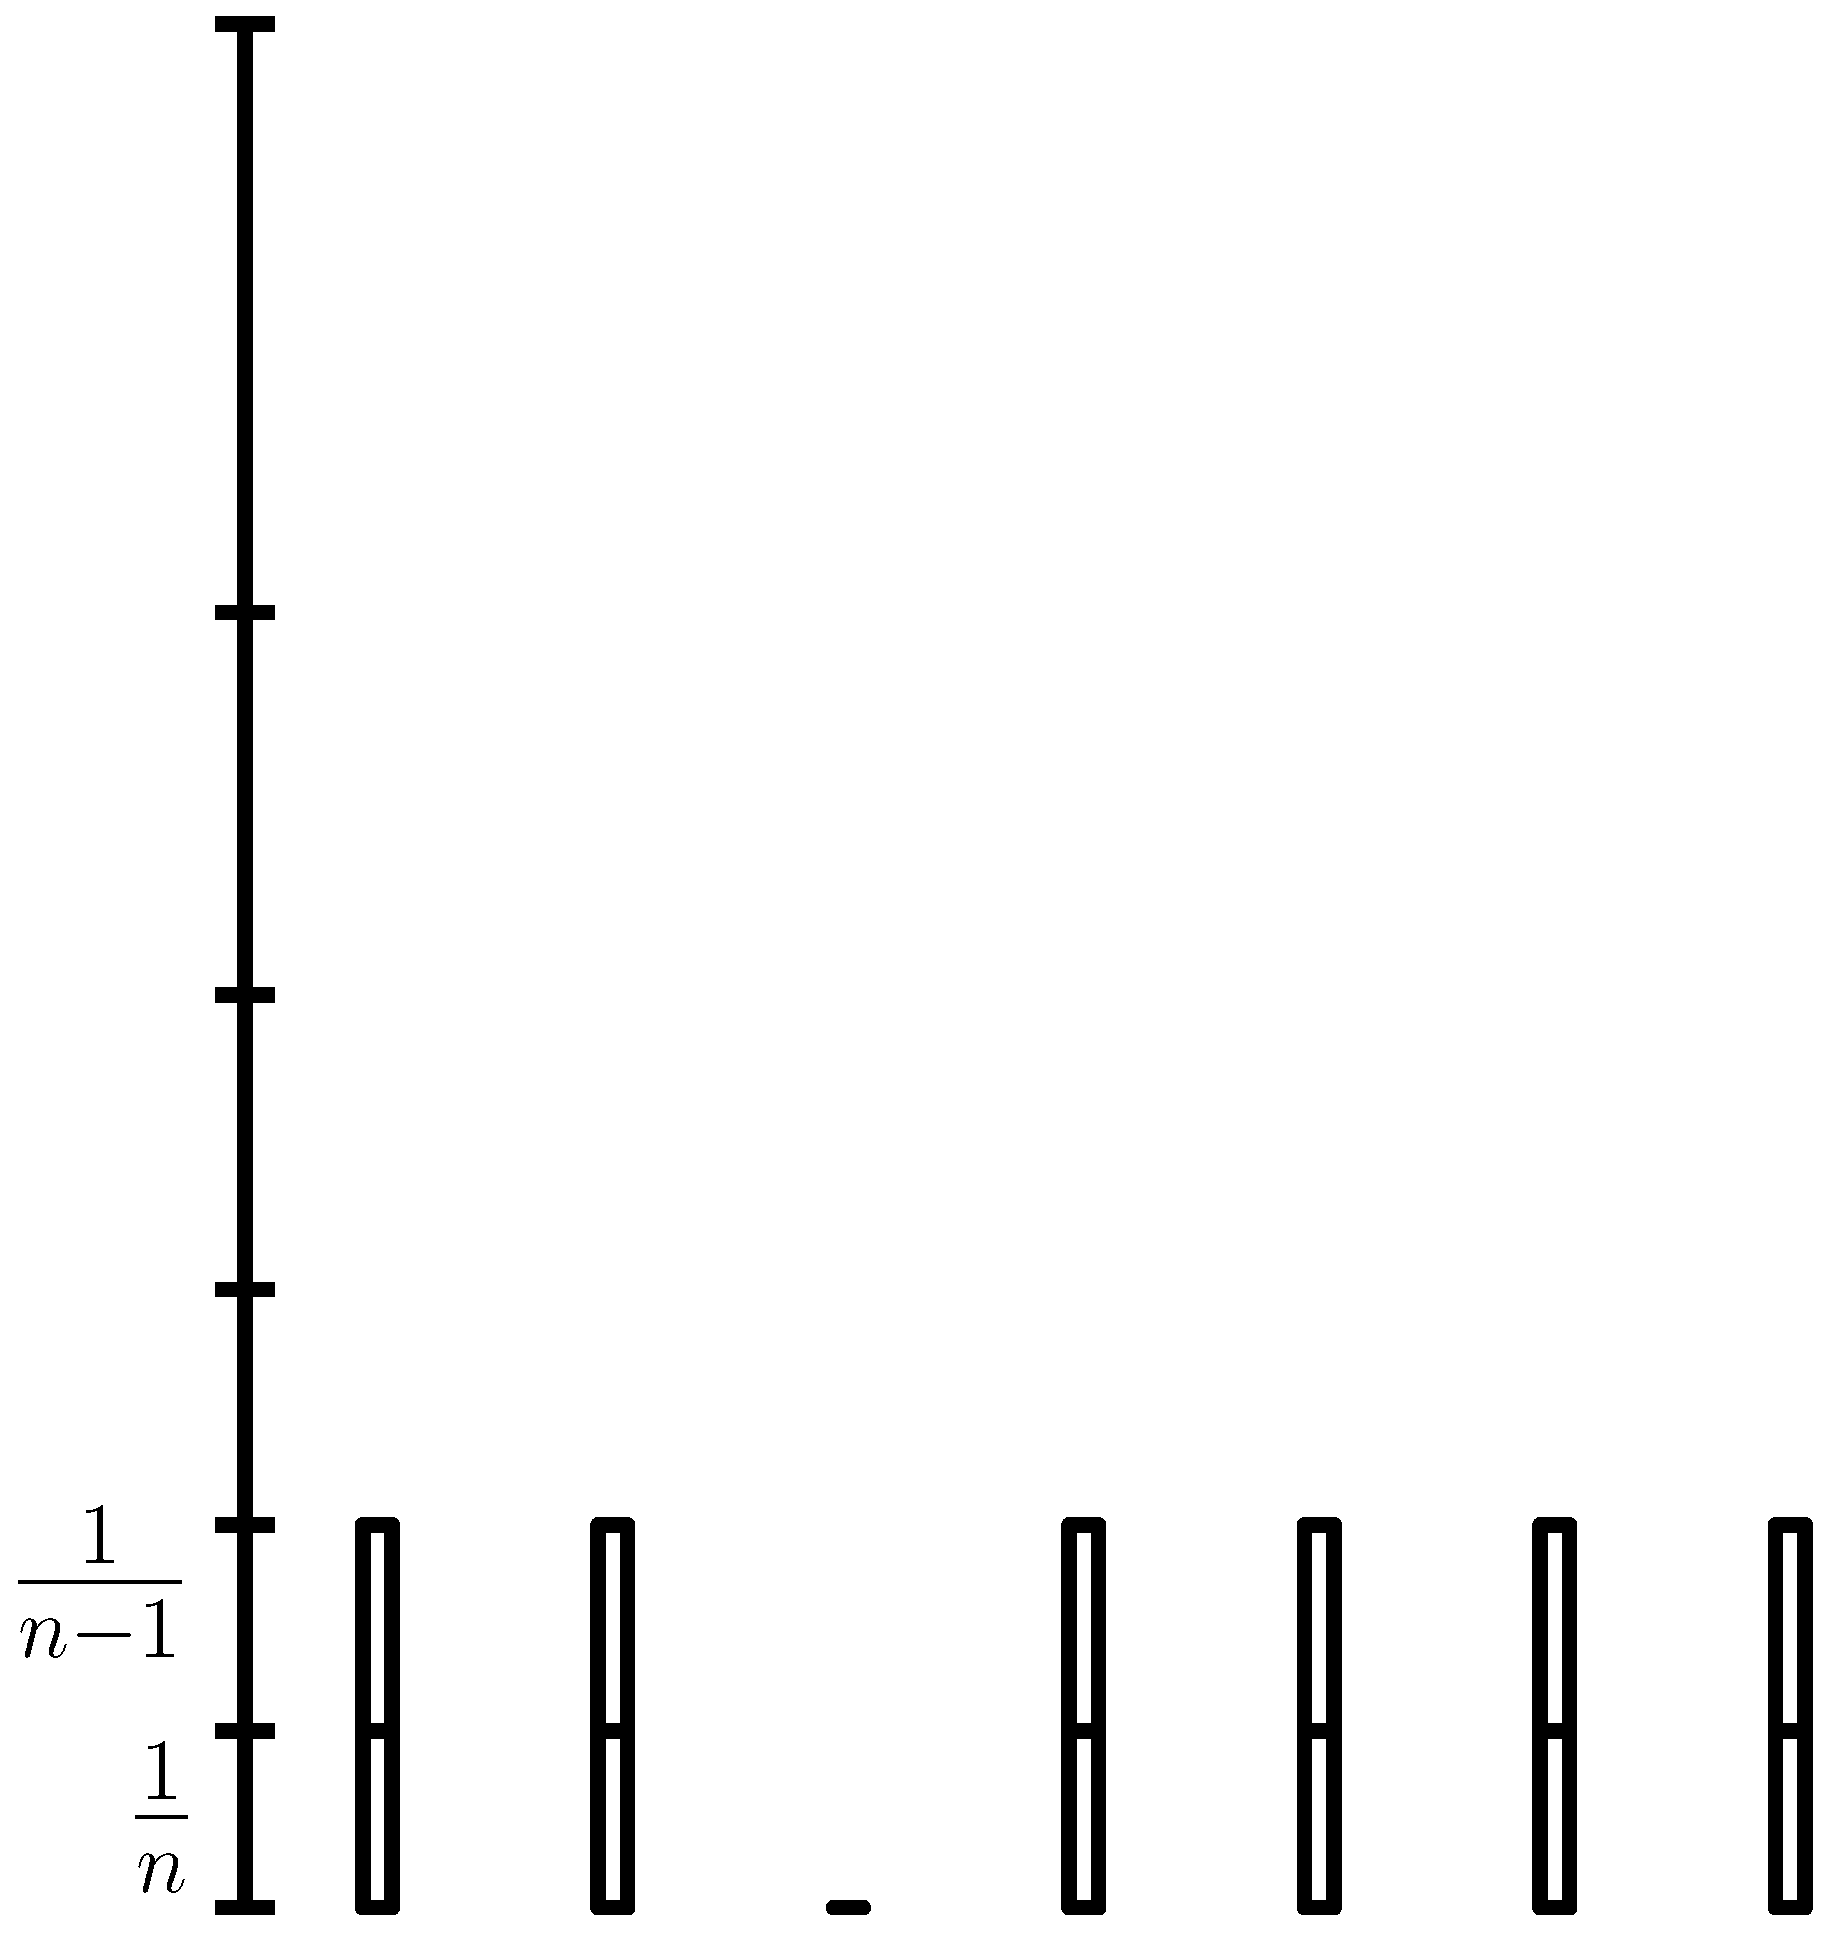
\includegraphics[width=0.5\linewidth]{singleProcessorLowerBound/round_2_0.eps}
    \onslide<5>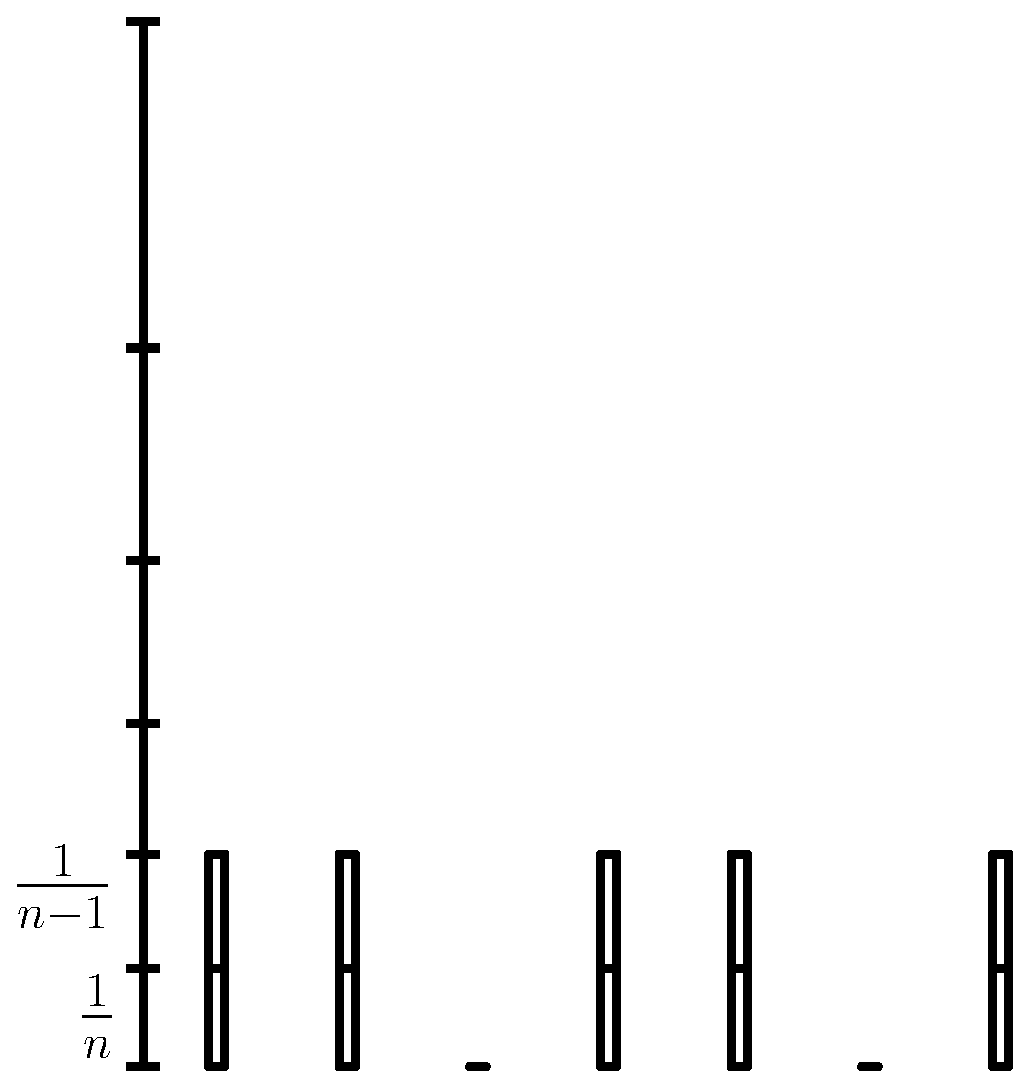
\includegraphics[width=0.5\linewidth]{singleProcessorLowerBound/round_2_1.eps}
    \onslide<6>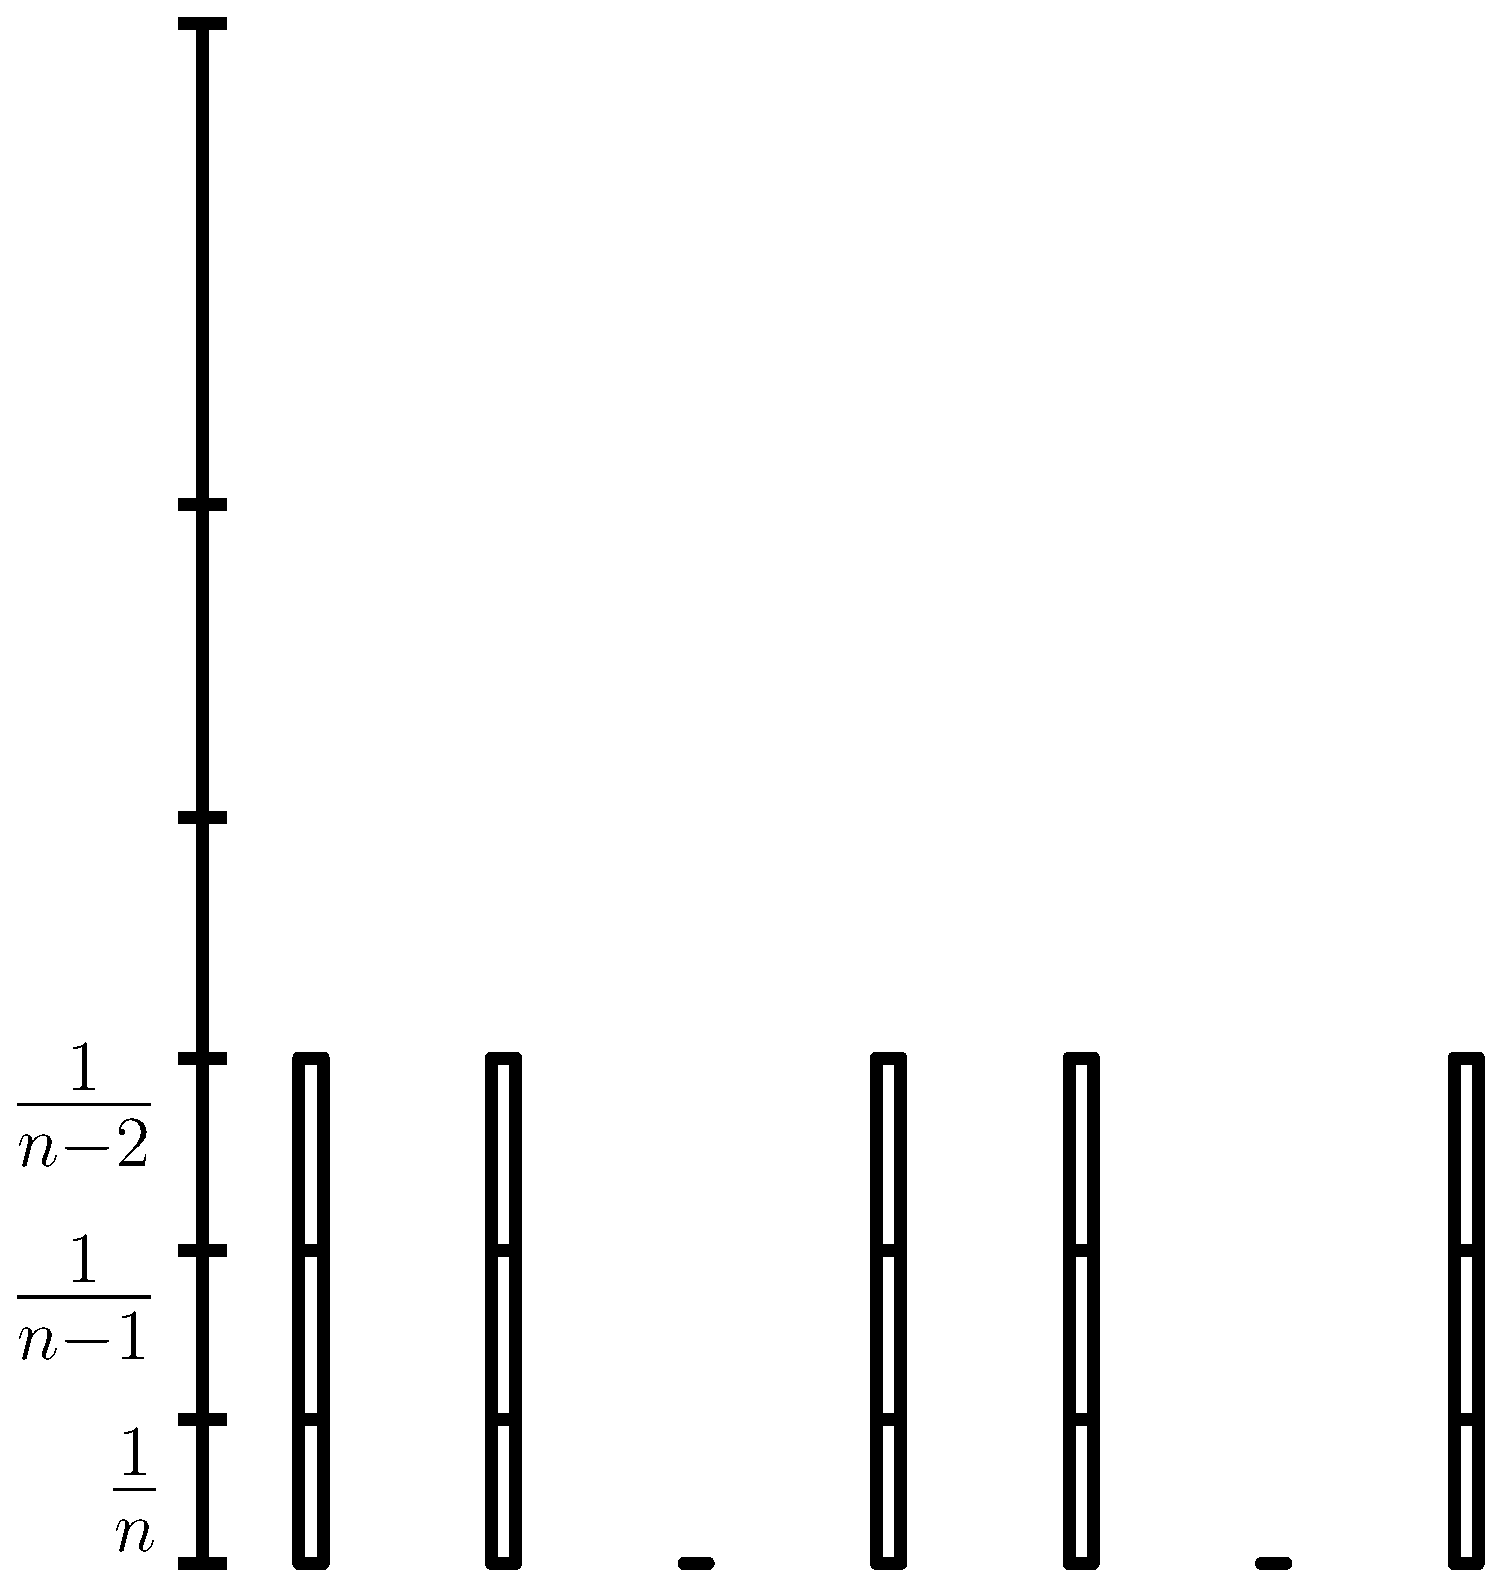
\includegraphics[width=0.5\linewidth]{singleProcessorLowerBound/round_3_0.eps}
    \onslide<7>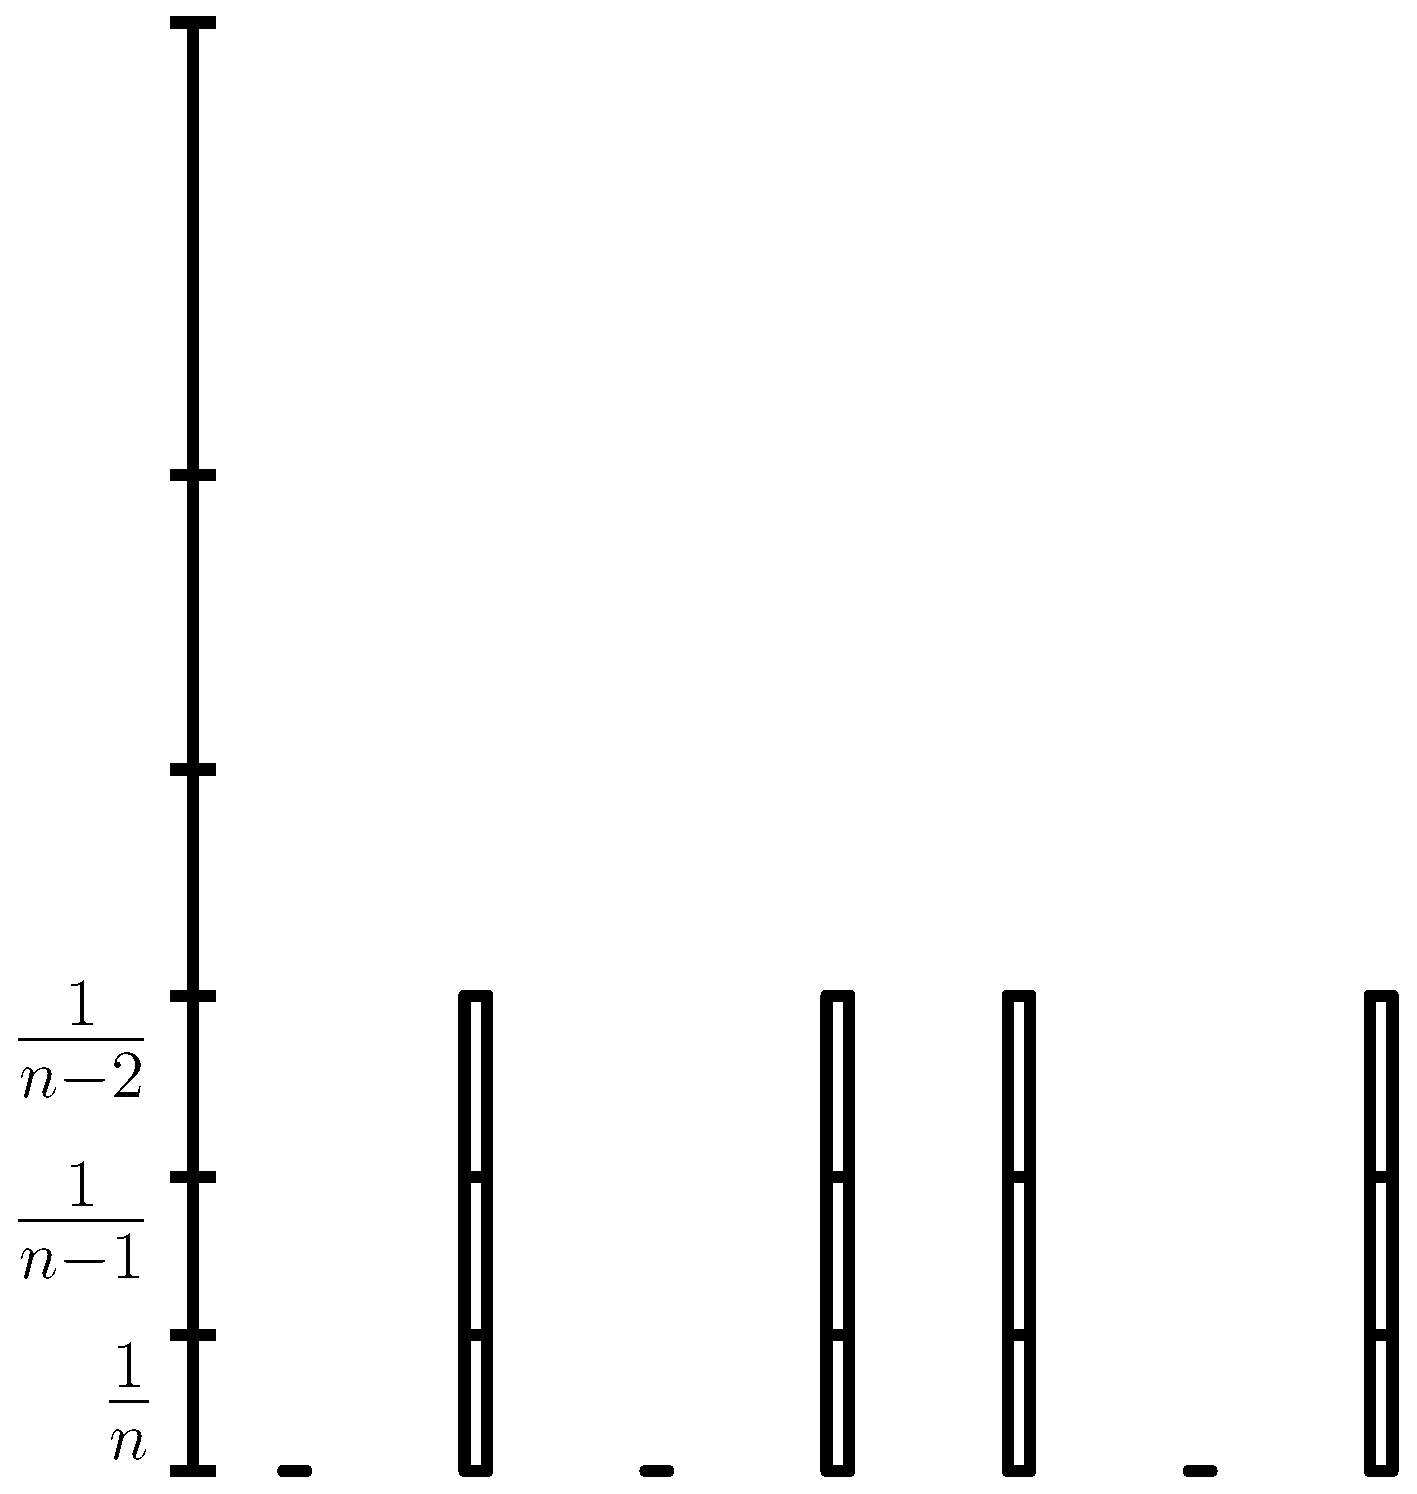
\includegraphics[width=0.5\linewidth]{singleProcessorLowerBound/round_3_1.eps}
    \onslide<8>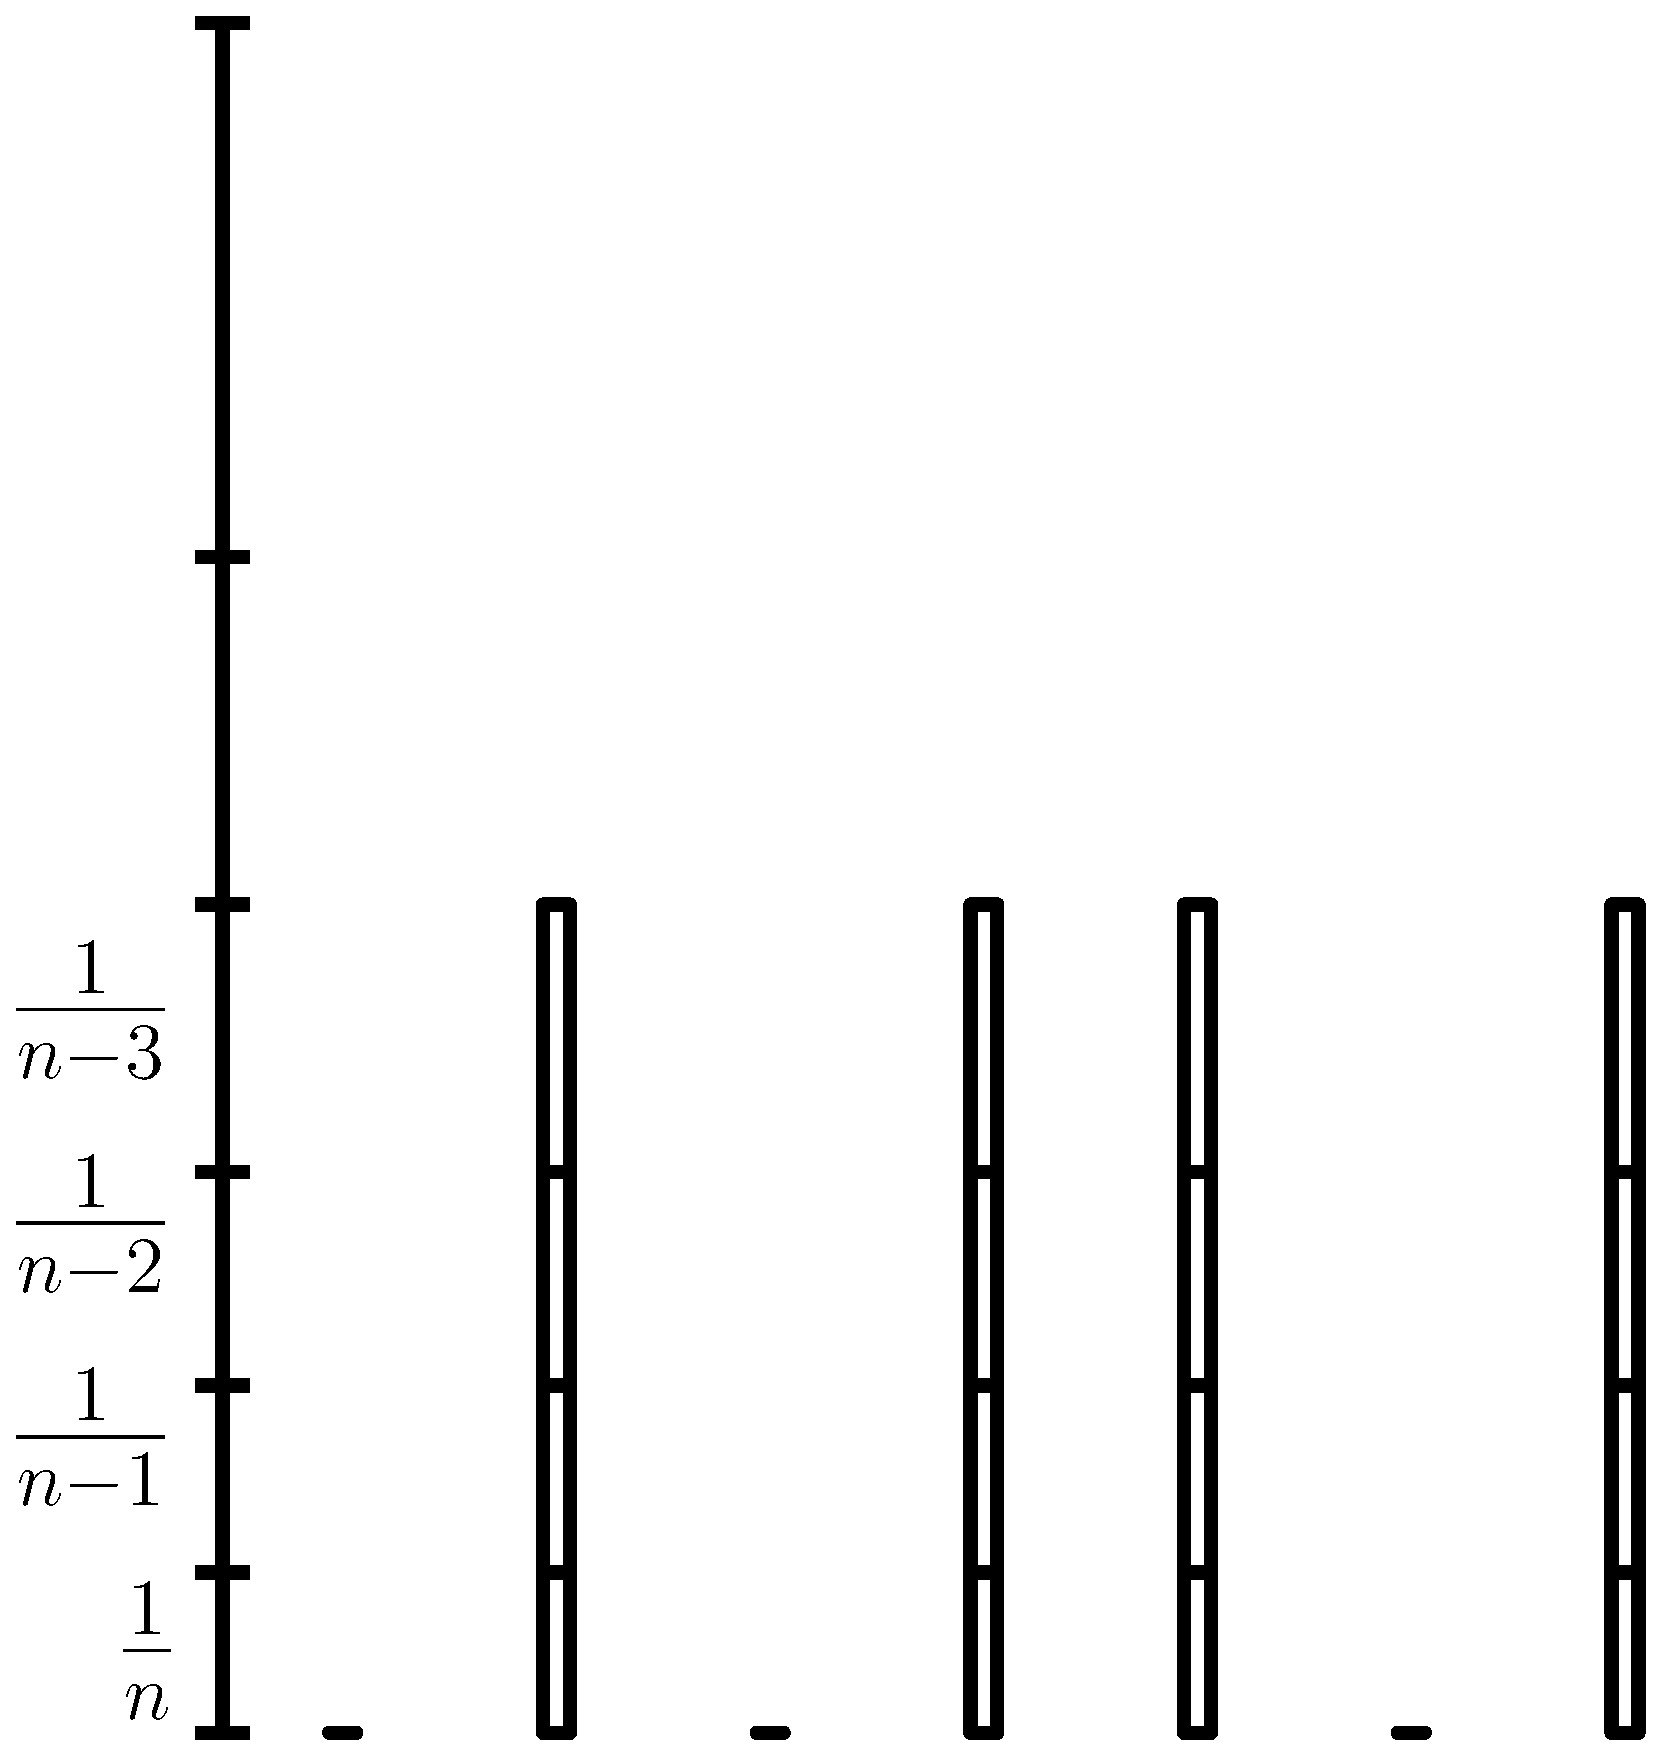
\includegraphics[width=0.5\linewidth]{singleProcessorLowerBound/round_4_0.eps}
    \onslide<9>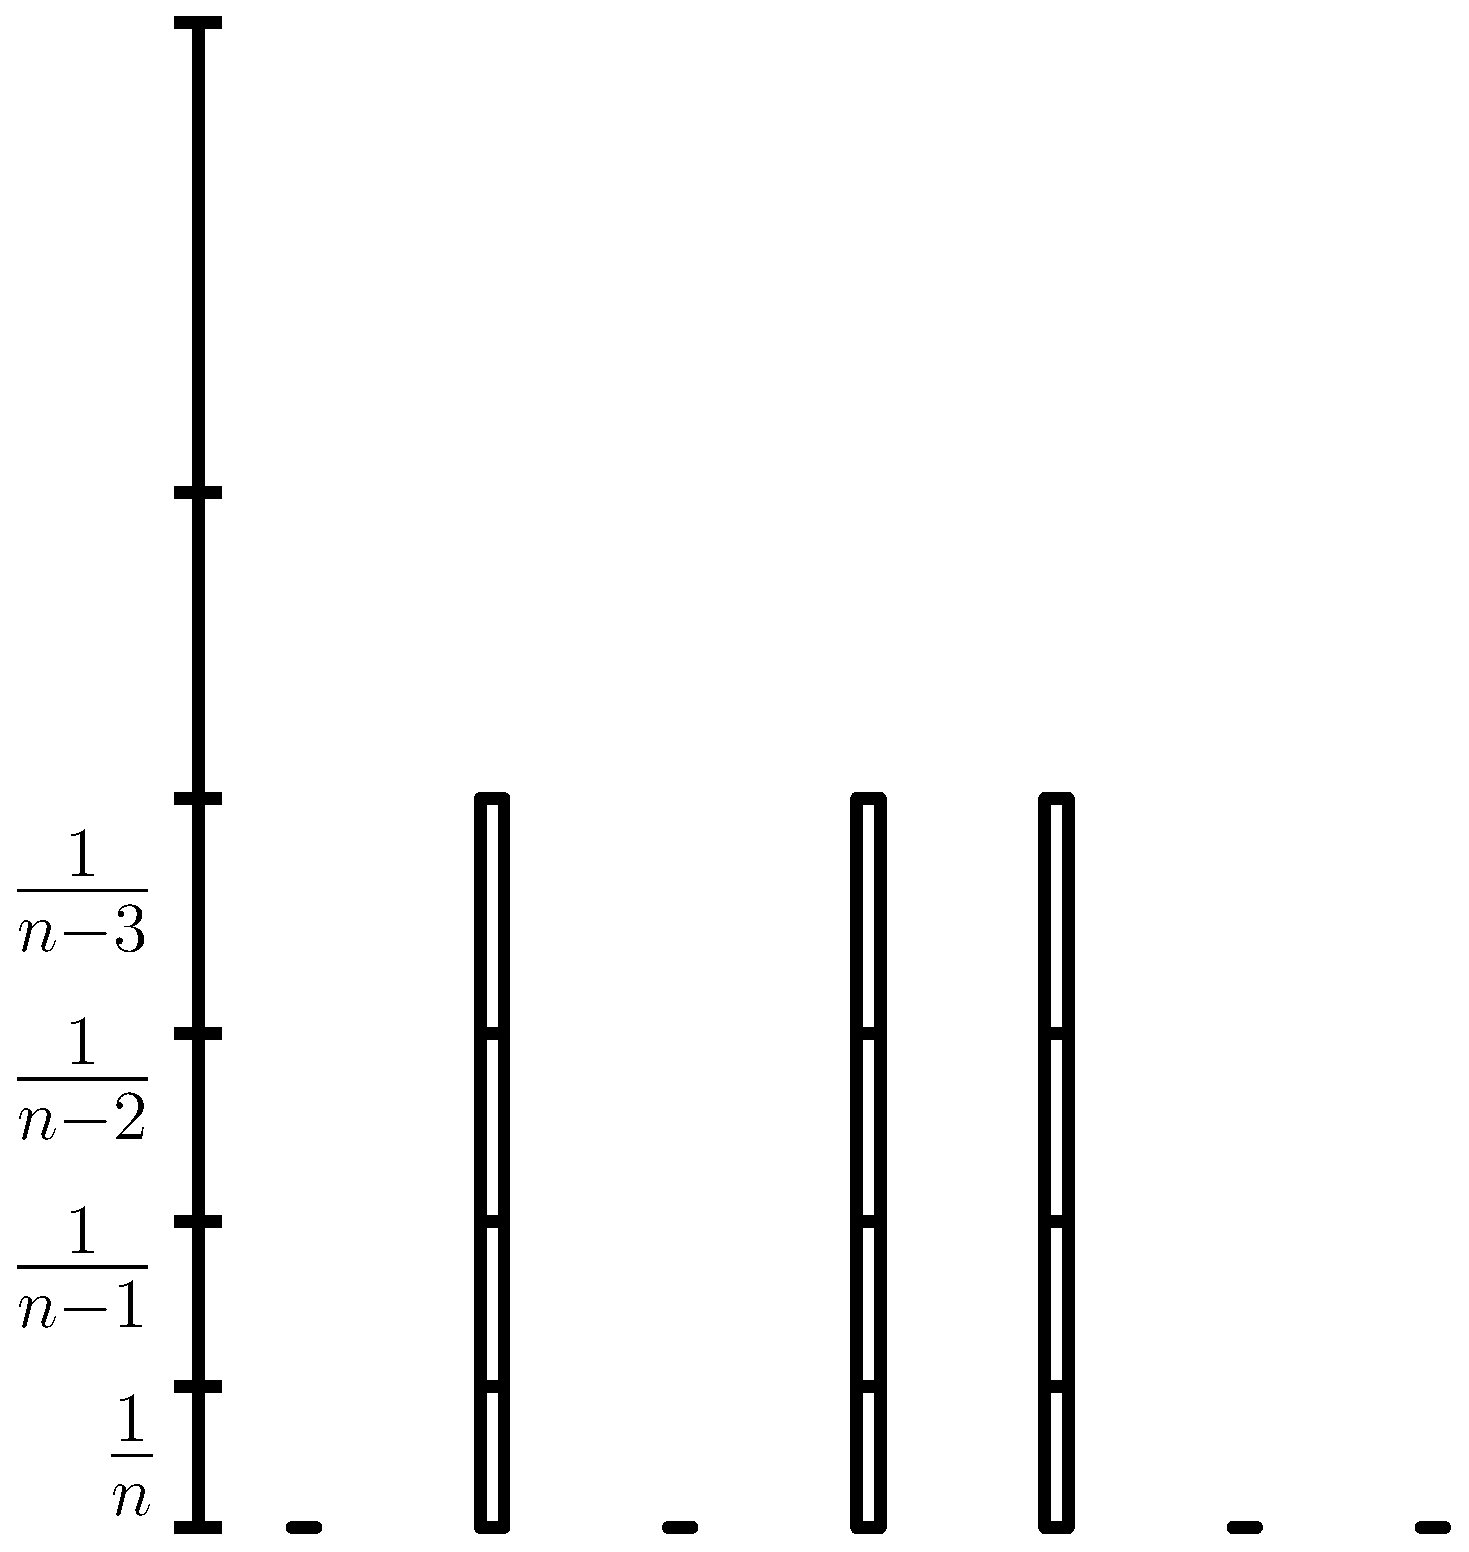
\includegraphics[width=0.5\linewidth]{singleProcessorLowerBound/round_4_1.eps}
    \onslide<10>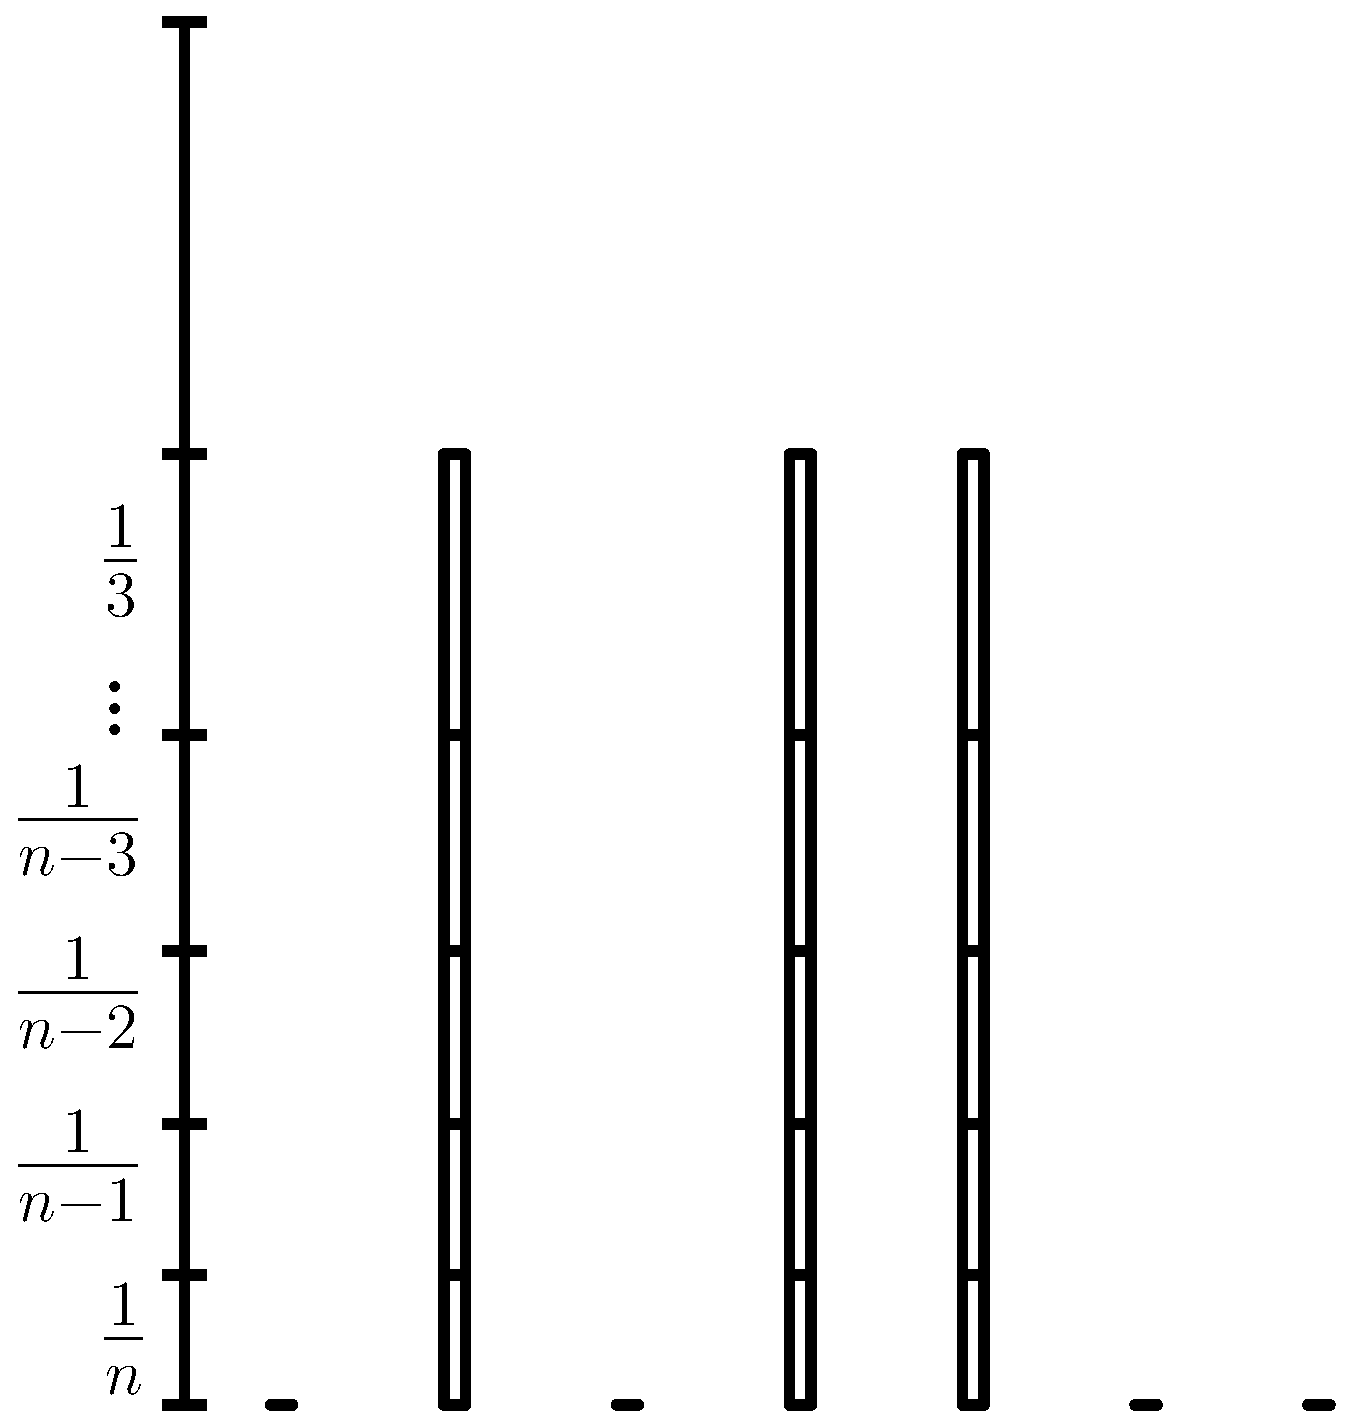
\includegraphics[width=0.5\linewidth]{singleProcessorLowerBound/round_5_0.eps}
    \onslide<11>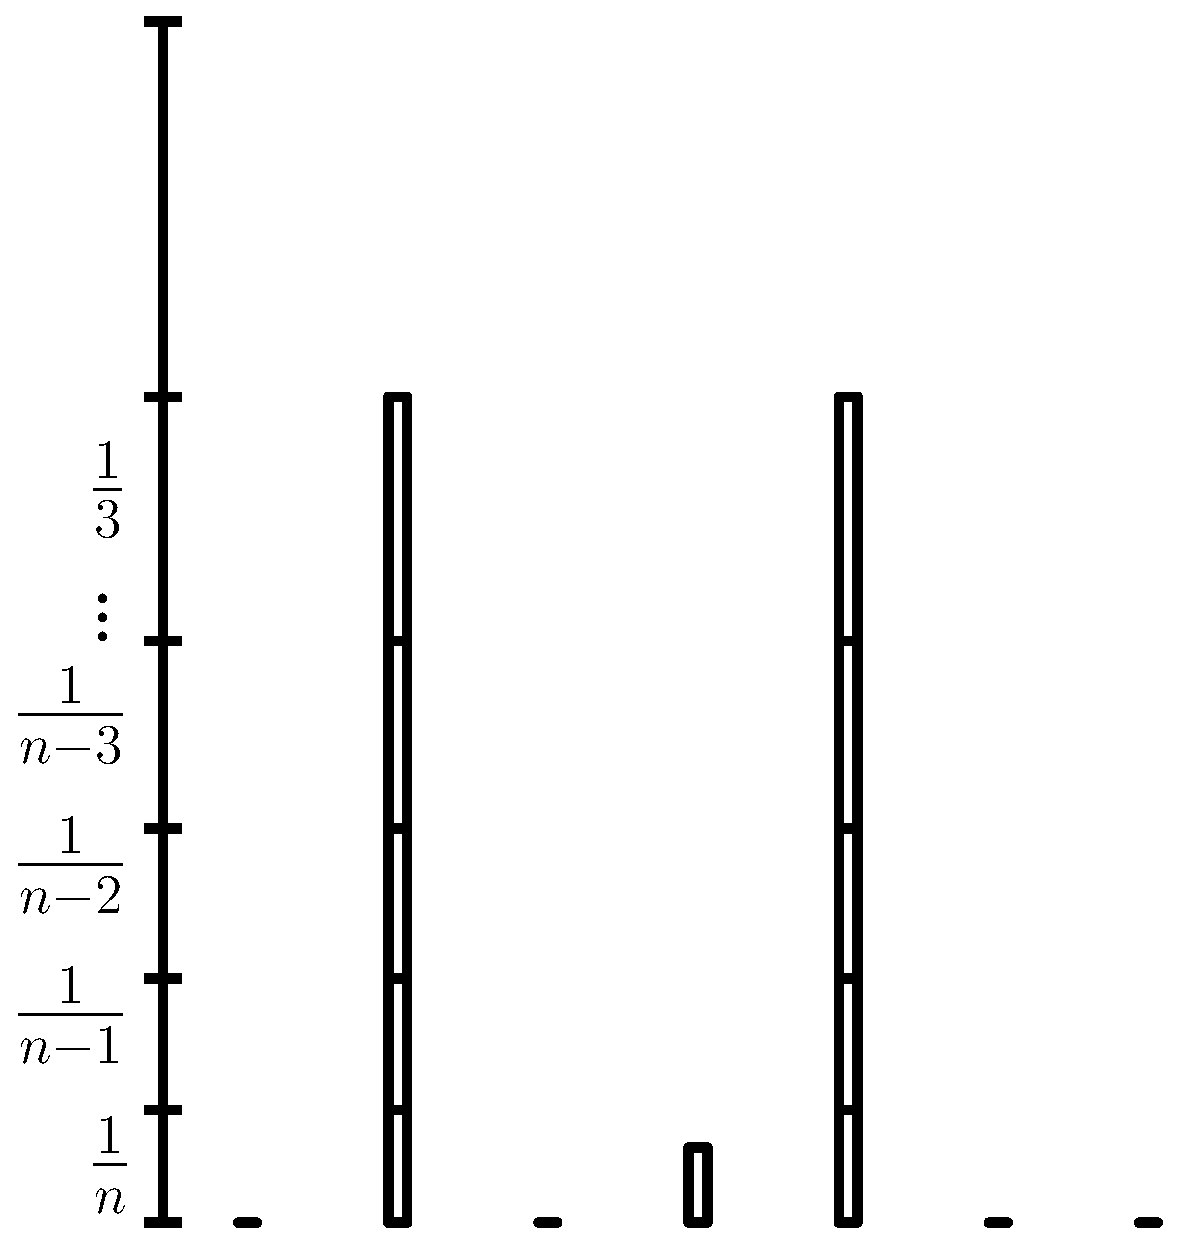
\includegraphics[width=0.5\linewidth]{singleProcessorLowerBound/round_5_1.eps}
    \onslide<12>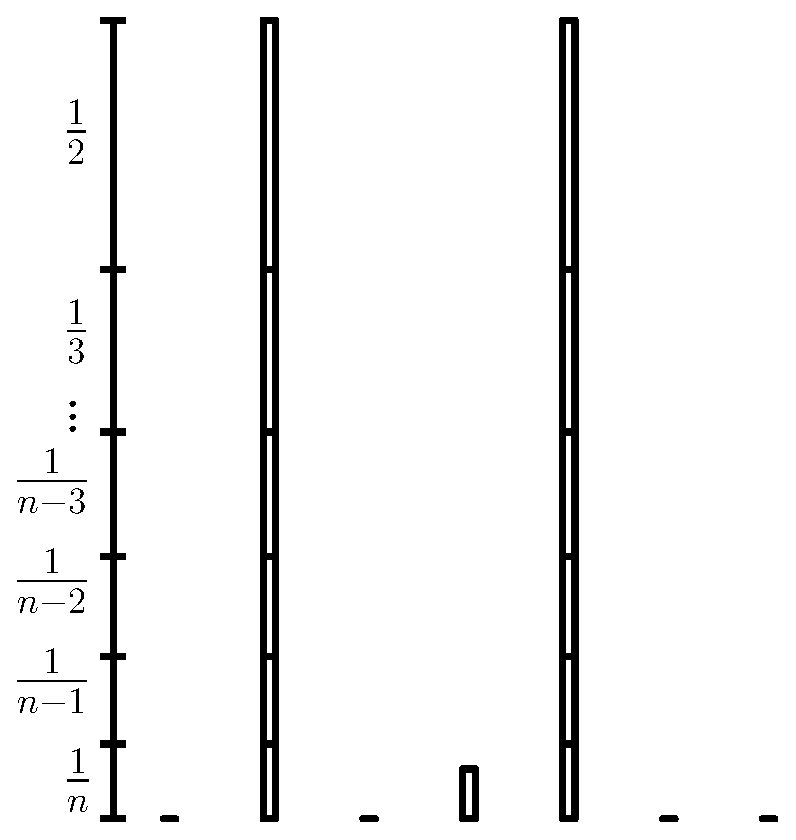
\includegraphics[width=0.5\linewidth]{singleProcessorLowerBound/round_6_0.eps}
    \onslide<13>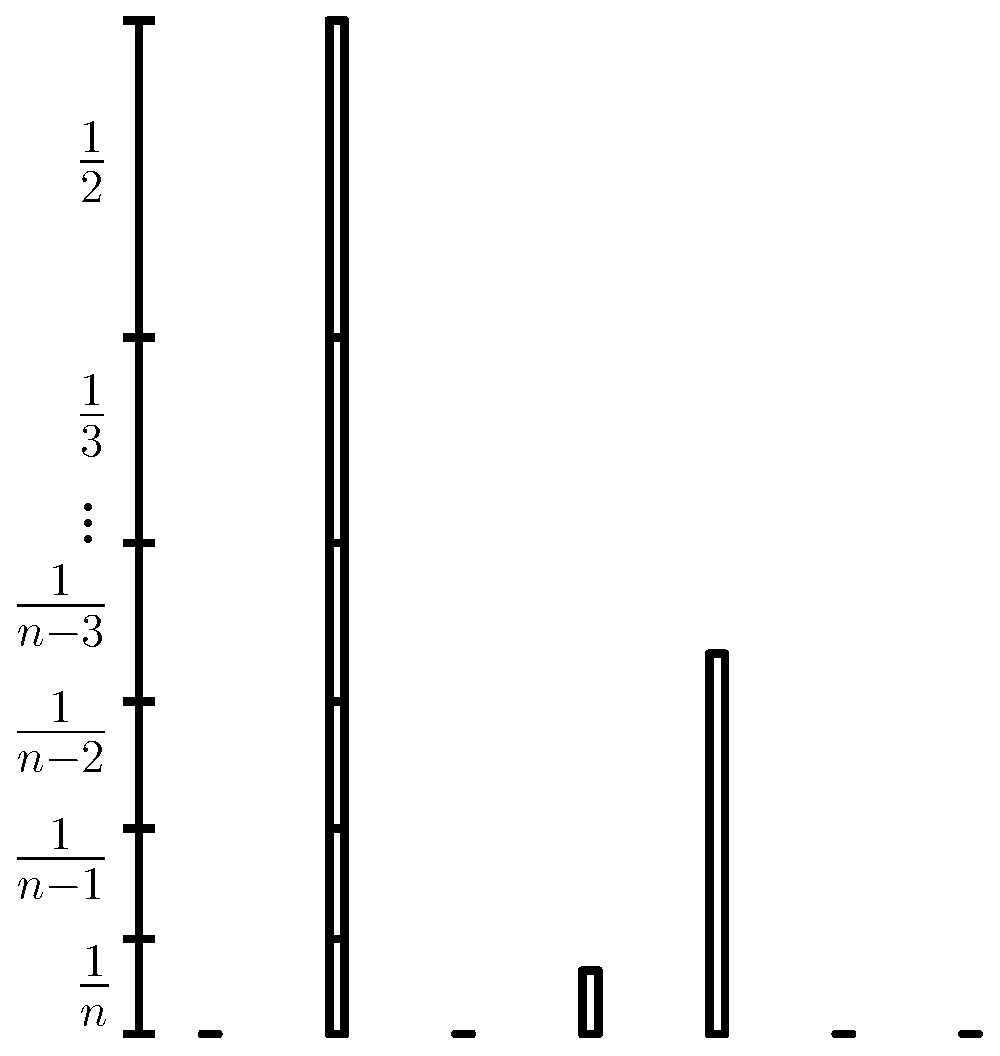
\includegraphics[width=0.5\linewidth]{singleProcessorLowerBound/round_6_1.eps}
    \onslide<14>\vspace{1.5cm}Achieves backlog: $$\frac{1}{n} + \frac{1}{n-1} + \cdots + \frac{1}{2} = \Omega(\log n).$$ 
  \end{overprint}
\end{frame}

\begin{frame}[t]{Single-Processor Upper Bound}
  A \defn{greedy emptier} -- an emptier that always empties from the
    fullest cup -- never lets backlog exceed $O(\log n)$.

  \vspace{0.75cm}
  \begin{definitions}
  \begin{itemize}
    \item $S_t$: state at start of round $t$
    \item $I_t$: state after the filler adds water on round $t$, but before the emptier removes water
    \item $\mu_k(S)$: average fill of $k$ fullest cups at state $S$.
  \end{itemize}
  \end{definitions}
\end{frame}

\begin{frame}[t]{Single-Processor Upper Bound Proof}
  \textbf{Proof:}
  Inductively prove a set of invariants: 
    $$\mu_k(S_t) \le \frac{1}{k+1} + \ldots +\frac{1}{n}.$$

  \vspace{0.25cm}
  Let $a$ be the cup that the emptier empties from on round $t$

  \vspace{0.25cm}
  \textbf{If $a$ is one of the $k$ fullest cups in $S_{t+1}$:}
  $$\mu_k(S_{t+1}) \le \mu_k(S_t).$$
  \textbf{Otherwise:}
  $$\mu_k(S_{t+1}) \le \mu_{k+1}(I_t) \le \mu_{k+1}(S_{t+1}) + \frac{1}{k+1}.$$
\end{frame}

% \begin{frame}[t]{Previous work on Cup Games}
%   \begin{itemize}
%     \item The Single-Processor cup game ($p=1$) has been tightly analyed with
%       \defn{oblivious} and \defn{adaptive} fillers (i.e. fillers that can't and
%       can observe the emtpier's actions).
%     \item The Multi-Processor cup game ($p>1$) is substantially more difficult. With an adaptive filler:
%       \begin{itemize}
%         \item Kuszmaul established upper bound of $O(\log n)$.\footnote{\tiny\color{blue}William Kuszmaul. Achieving optimal backlog in the vanilla multi-processor cup game. SIAM, 2020.}
%         \item We established a matching lower bound of $\Omega(\log n)$.
%       \end{itemize}
%     \item The multi-processor cup game with an oblivious filler has not yet
%       been tightly analyzed.
%     \item Variants where valid moves depend on a graph have been studied.
%     \item Variants with resource augmentation have been studied.
%     \item Variants with clairvoyance have been studied.
%   \end{itemize}
% \end{frame}

\begin{frame}[t]{Our Variant of the Cup Game}
We analyzed a new variant of the classic multi-processor cup game,
the \defn{variable-processor cup game}, in which \emph{the resources are variable}:
the filler is allowed to change $p$.

\vspace{1cm}
Specifically we found upper bounds and lower bounds on backlog with oblivious
and adaptive fillers.

\vspace{1cm}
The modification to allow variable resources may seem small. However, we show
that it drastically changes the game. 
\end{frame}

\begin{frame}[c]{}
\begin{center}
\Huge Adaptive Filler\\ Lower Bound
\end{center}
\end{frame}

\begin{frame}[t]{Negative Fill}
  In lower bound proofs we allow \defn{negative fill}
  \begin{itemize}
    \item We measure fill relative to average fill
    \item Important for recursion 
    \item Game is strictly easier for the filler if cups can zero out
  \end{itemize}
\end{frame}

\begin{frame}[t]{Amplification Lemma}
  \begin{lemma}
    Given a strategy $f$, we can construct a new strategy that achieves backlog 
    $$f'(n) \ge (1-\delta)\sum_{\ell=0}^L f((1-\delta)\delta^\ell n)$$
    for appropriate parameters $L\in\mathbb{N}, 0<\delta\ll 1/2$.
  \end{lemma}
\end{frame}

\begin{frame}[t]{Amplification Lemma Proof Sketch}
  \begin{itemize}
    \item $A$ starts as the $\delta n$ fullest cups, $B$ as the $(1-\delta)n$ other cups.
    \item Repeatedly apply $f$ to $B$ and swap the cup with fill increased by $f((1-\delta)n)$ into $A$. 
    \item Recurse on $A$, filler will decrease $p$.
  \end{itemize} 
  \vspace{0.5cm}
  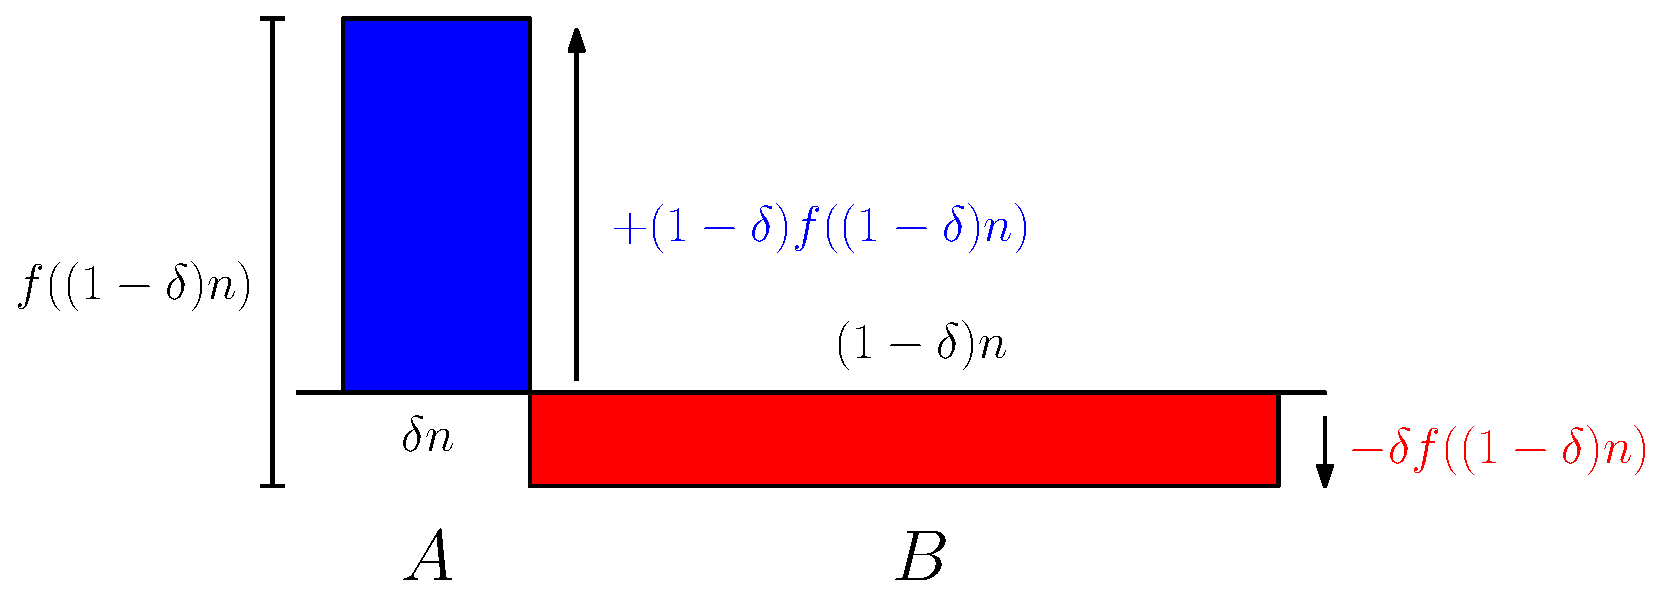
\includegraphics[width=\linewidth]{amplificationImgs/delta_one_minus_delta.eps}
\end{frame}

\begin{frame}[t]{Adaptive Filler Lower Bound}
  By repeated amplification, using $\delta=\Theta(1)$, we get: 
  \begin{theorem}
    There is an adaptive filling strategy that achieves
    backlog $\Omega(n^{1-\epsilon})$ for constant
    $\epsilon > 0$ of our choice in running-time $2^{O(\log^2 n)}$.
  \end{theorem}
  \vspace{0.5cm}
  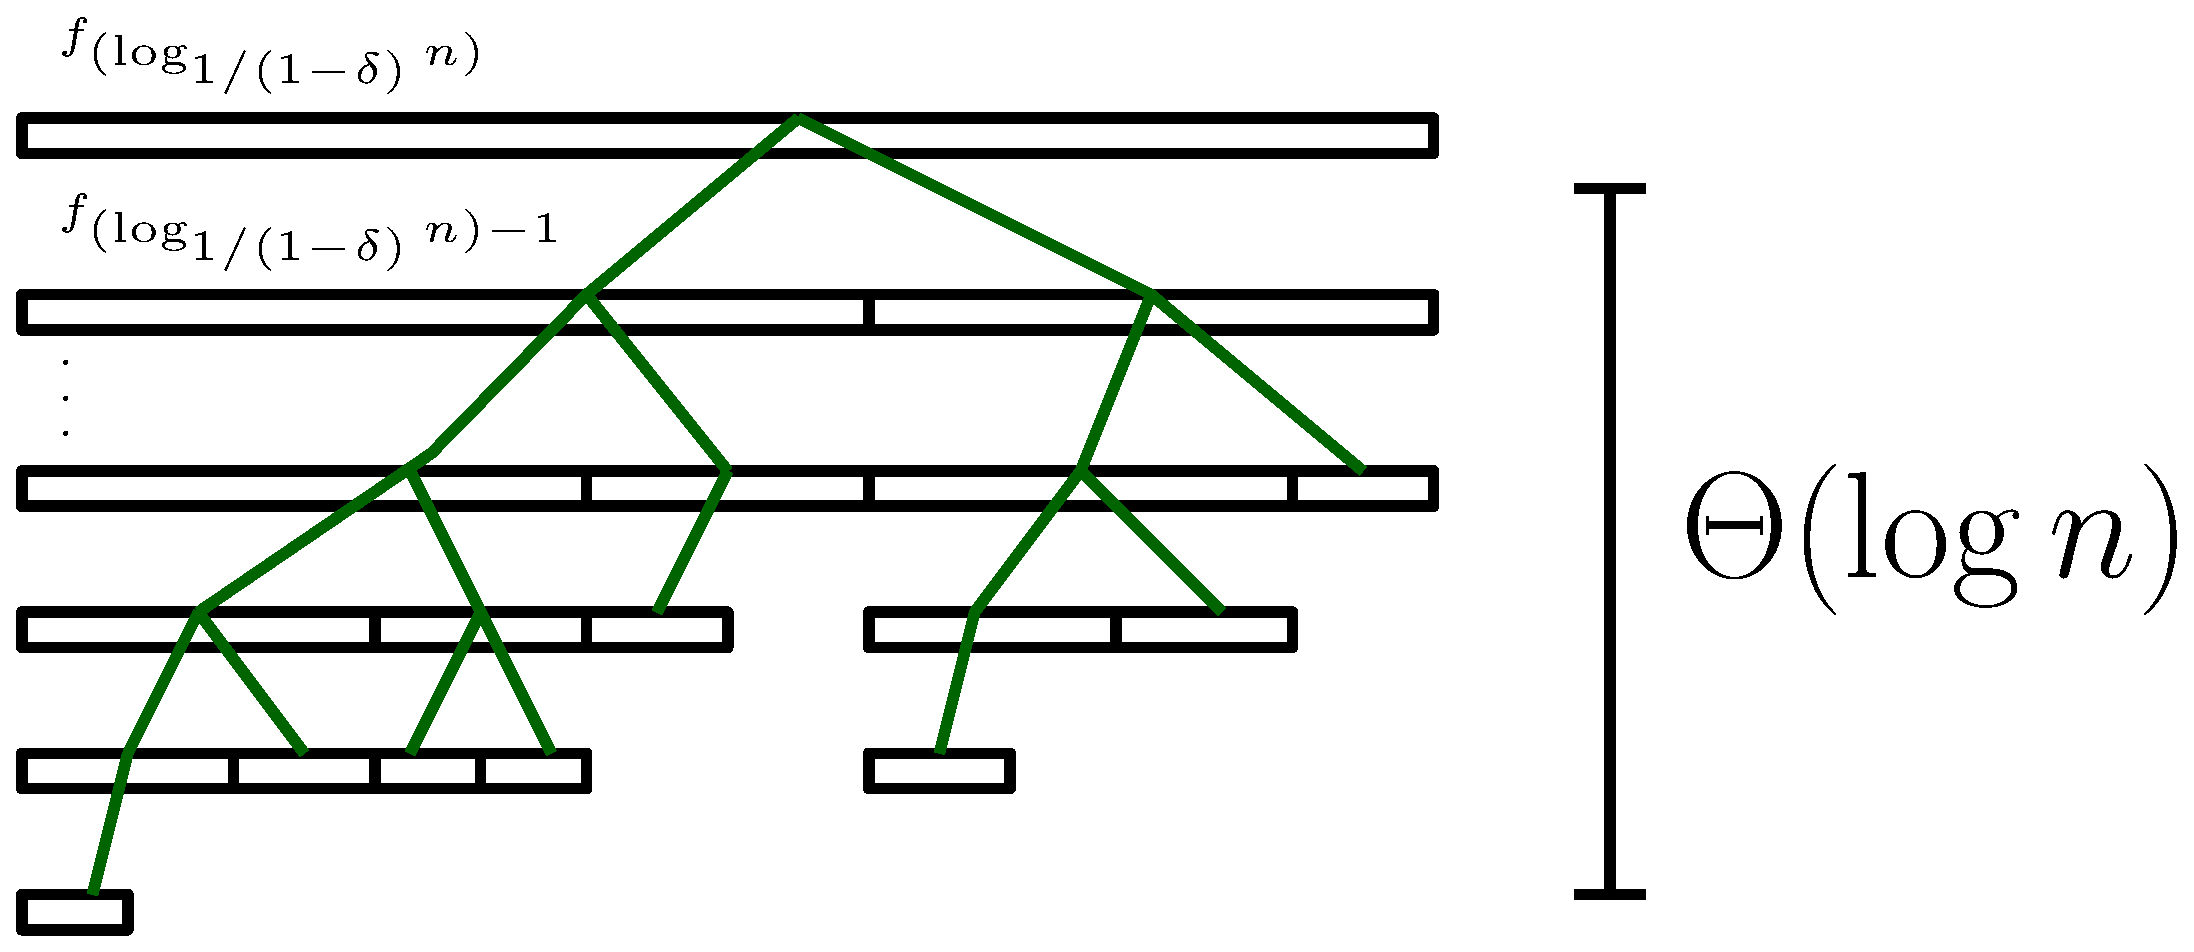
\includegraphics[width=0.7\linewidth]{amplificationImgs/quasipoly_cor.eps}
\end{frame}

\begin{frame}[t]{Adaptive Filler Lower Bound}
  By repeated amplification, using $\delta=\Theta(1/n)$, we get: 
  \begin{theorem}
    There is an adaptive filling strategy that achieves backlog $\Omega(n)$ in running-time $2^{O(n)}$.
  \end{theorem}
  \vspace{0.5cm}
  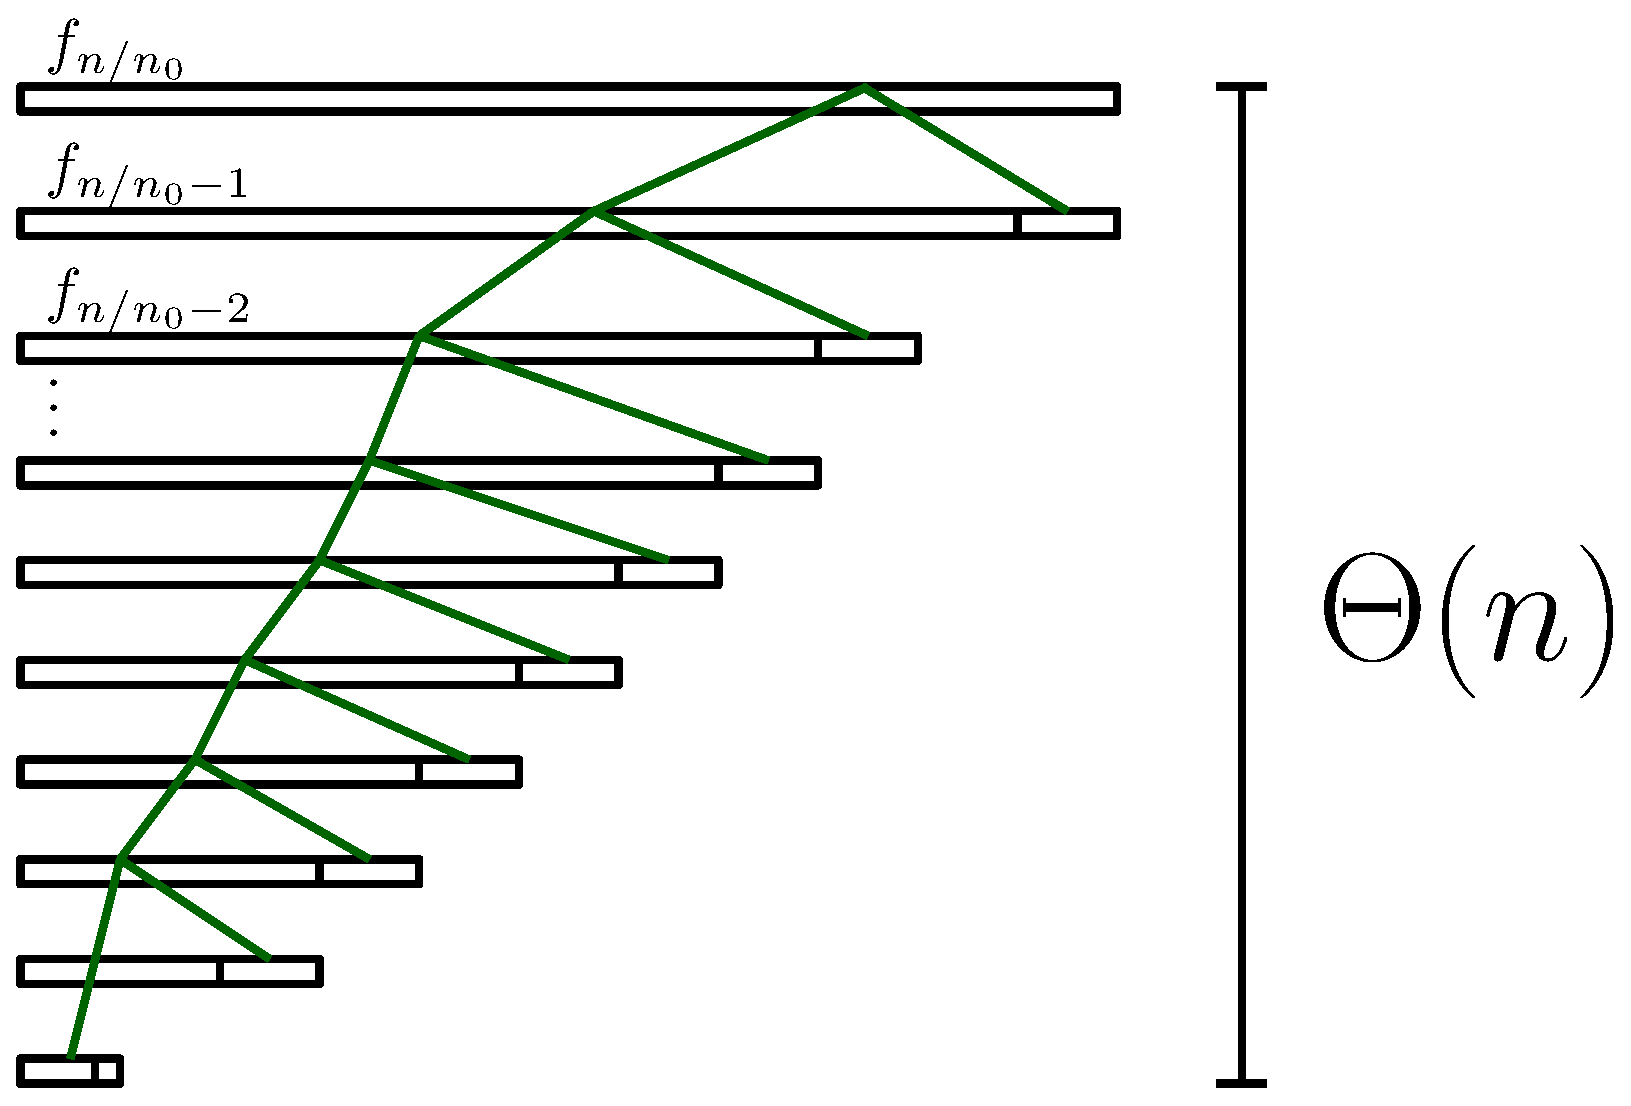
\includegraphics[width=0.45\linewidth]{amplificationImgs/expo_cor.eps}
\end{frame}

\begin{frame}[c]{}
  \begin{center}
    \Huge Upper Bound 
  \end{center}
\end{frame}

\begin{frame}[t]{Upper Bound}
  We prove a novel set of invariants:

  \begin{theorem}
    A greedy emptier maintains the invariant:
    $$\mu_k(S_t) \le 2n-k.$$
  \end{theorem}

  \vspace{0.3cm}
  In particular this implies that backlog is $$O(n).$$

  \vspace{0.3cm}
  Note: this matches our lower bound!
\end{frame}

\begin{frame}[t]{Upper Bound Proof Sketch}
  Extremal fill configuration:
  \vspace{0.5cm}
  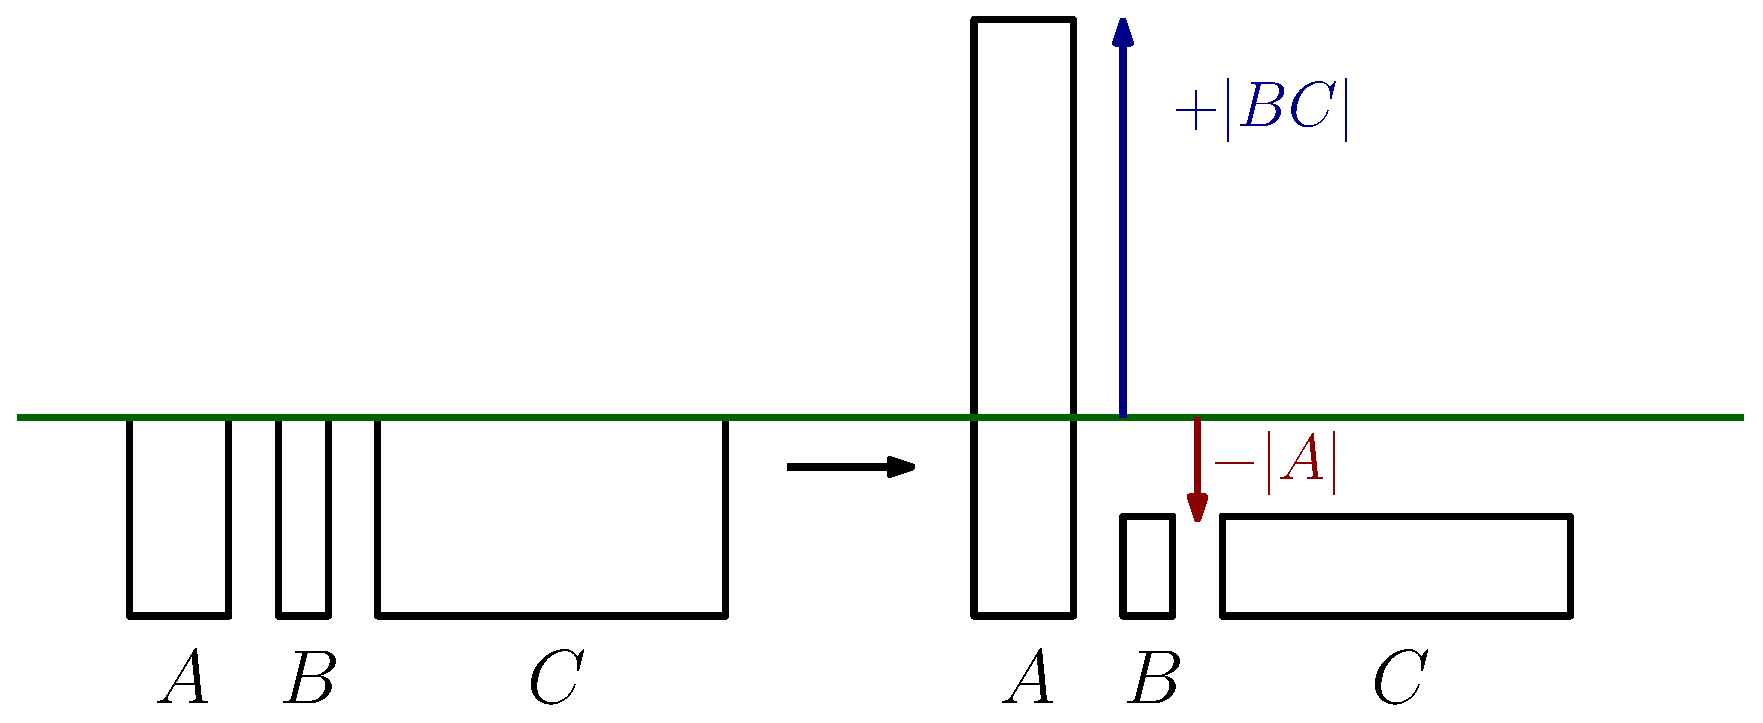
\includegraphics[width=\linewidth]{upperbound/upperboundpf.eps}
\end{frame}

\begin{frame}[c]{}
  \begin{center}
    \Huge Oblivious Filler \\
    Lower Bound
  \end{center}
\end{frame}

\begin{frame}[t]{Oblivious Filler Lower Bound}
  \vspace{0.5cm}
  Classically emptier does much better in the randomized setting.

  \vspace{0.5cm}

  But not in the variable-processor cup game!

  \vspace{0.5cm}
  In the variable-processor cup game, an oblivious filler do essentially just
  as well as teh adaptive filler, although we only are able to analyze it with
  \defn{greedy-like emptiers}. 

  % In the variable-processor cup game--shockingly--an oblivious filler can
  % achieve an identical lower bound for games of length $2^{\polylog(n)}$ 
  % with probability at least $1-2^{-\polylog(n)}$, although only against \defn{greedy-like} emptiers.
\end{frame}

\begin{frame}[t]{Oblivious Filler: Constant Fill}
  Getting constant fill in a \emph{known} cup is hard now. Strategy:
  \begin{itemize}
    \item Play lots of single-processor cup games on constant numbers of cups
      blindly. Each succeeds with some constant probability.
    \item By a Chernoff Bound, with \emph{exponentially} good probability, i.e.
      $1-2^{-\Omega(n)}$, at least a constant fraction, say $nc$, of the single-processor
      cup games succeed.
    \item Set $p=nc$.
    \item Exploiting the greedy-like nature of the emptier fill a set of $nc$
      known cups while the emptier is forced to focus on the set of $nc$ with
      high fill.
    \item Recurse for a constant number of levels on the $nc$ cups with known high fill. 
  \end{itemize}
\end{frame}

\begin{frame}[t]{Oblivious Amplification Lemma}
Almost identical to the Adaptive Amplification Lemma!
  \begin{lemma}
    Given a strategy $f$, we can construct a new strategy that achieves backlog 
    $$f'(n) \ge \phi \cdot (1-\delta)\sum_{\ell=0}^L f((1-\delta)\delta^\ell n)$$
    for appropriate parameters $L\in\mathbb{N}, 0<\delta\ll 1/2$ and constant $\phi \in (0,1)$ of our choice.
  \end{lemma}

  (Note: Lemma is actually more complicated than this.)
\end{frame}

\begin{frame}[t]{Oblivious Filler Lower Bound }
  \begin{theorem}
    There is an oblivious filling strategy that achieves backlog
    $$\Omega(n^{1-\epsilon})$$ for constant $\epsilon > 0$ with probability at
    least $1-2^{-\polylog(n)}$ in running time $2^{O(\log^2 n)}$.
  \end{theorem}

  \vspace{0.5cm}
  Proof notes: 
  \begin{itemize}
    \item Similar to adaptive filler proof
    \item need larger base case for union bound to work; this doesn't harm backlog though
  \end{itemize}
\end{frame}

\begin{frame}[t]{Open Questions}
  \begin{itemize}
    \item Can we extend the Oblivious lower-bound construction to work with arbitrary emptiers?
    \item Are there shorter more simple constructions?
  \end{itemize}
\end{frame}

\begin{frame}[t]{Acknowledgements}
  \begin{itemize}
    \item My mentor, William Kuszmaul!
    \item MIT PRIMES
    \item My Parents
 \end{itemize} 
\end{frame}

\end{document}
